%% ============================================================
%% MALTG-SDS — Artículo científico formato MDPI (revista Computers)
%% Compilar: pdflatex paper && bibtex paper && pdflatex paper && pdflatex paper
%% ============================================================
\documentclass[computers,article,submit,pdftex,moreauthors]{Definitions/mdpi}

%% Paquetes para figuras y matemáticas
\usepackage{tikz}
\usetikzlibrary{arrows.meta,positioning,shapes.geometric,fit,backgrounds,calc}
\usepackage{pgfplots}
\pgfplotsset{compat=1.17}
\usepgfplotslibrary{polar}

%% Castellanización de etiquetas de flotantes
\renewcommand{\figurename}{Figura}
\renewcommand{\tablename}{Tabla}

%% Metadatos del número (placeholder de envío)
\firstpage{1}
\makeatletter
\setcounter{page}{\@firstpage}
\makeatother
\pubvolume{15}
\issuenum{1}
\articlenumber{0}
\pubyear{2026}
\copyrightyear{2026}
\datereceived{ }
\daterevised{ }
\dateaccepted{ }
\datepublished{ }

%% ── Título (mejorado) ──────────────────────────────────────
\Title{MALTG-SDS: Arquitectura de Sombra Digital Guiada por Ontologías para Ecosistemas LegalTech con Ingesta Semántica Automatizada de Datos Judiciales Públicos mediante JSON-LD y Validación por Cobertura Jerárquica}

%% ── Autoría (reemplazar con datos definitivos) ─────────────
\newcommand{\orcidauthorA}{0000-0000-0000-0000}
\Author{Patricio Michael~Autor $^{1,}$*}
\AuthorNames{Patricio Michael Autor}
\address{$^{1}$ \quad Programa de Doctorado / Facultad de Ingeniería; correo institucional}
\corres{Correspondencia: pat\_mic@hotmail.com}

%% ── Resumen ────────────────────────────────────────────────
\abstract{La transformación digital de los sistemas judiciales genera ecosistemas tecnológicos heterogéneos cuya madurez de gobernanza rara vez puede auditarse de forma automatizada, reproducible y fundamentada semánticamente. Este artículo propone MALTG-SDS, una arquitectura de \emph{sombra digital} (digital shadow) guiada por ontologías para ecosistemas LegalTech, que construye de manera automática una representación estructural en JSON-LD del ecosistema digital de una institución judicial a partir de sus datos públicos, y la evalúa contra una ontología de gobernanza multiestándar (TOGAF, COBIT, ITIL, NIST CSF y un dominio LegalTech específico). El enfoque se formaliza mediante la quíntupla $\mathcal{M} = \langle \Omega, \Delta, \Gamma, \Psi, \delta \rangle$, donde la función de cobertura jerárquica $\Psi$ cuantifica el grado en que la sombra digital materializa cada dimensión ontológica y la función de brecha $\delta$ prioriza la remediación. El módulo GET-SDS implementa un flujo no invasivo de adquisición de evidencia web, proyección semántica a JSON-LD y visualización mediante un grafo tridimensional interactivo. La arquitectura, contenedorizada con Docker, se valida con un caso de estudio sobre el Consejo de la Judicatura del Ecuador: la sombra digital generada (34 componentes, 32 flujos, 7 capas) arroja un índice de madurez de 46/100 (nivel 3, «Definido»), con la interoperabilidad semántica como dimensión más débil (28/100), y la validación sintética de diez dimensiones alcanza una cobertura global $\Psi$ del 90{,}5\% (66{,}9 frente a 73{,}9 puntos ontológicos). Los resultados muestran que las sombras digitales semánticas permiten auditorías de gobernanza continuas, trazables y comparables en el sector justicia.}

%% ── Palabras clave ─────────────────────────────────────────
\keyword{sombra digital; gemelo digital; ontologías; JSON-LD; LegalTech; gobierno electrónico; datos judiciales abiertos; web semántica; madurez digital; arquitectura de software}

\begin{document}

%% ============================================================
\section{Introducción}
\label{sec:intro}

Los sistemas judiciales de América Latina, y en general del mundo, atraviesan procesos de digitalización acelerada que combinan portales institucionales, sistemas de gestión procesal, servicios de consulta ciudadana y repositorios estadísticos. El resultado es un ecosistema tecnológico heterogéneo en el que conviven arquitecturas modernas de una sola página (SPA), gestores de contenido genéricos y aplicaciones heredadas (\emph{legacy}), con niveles de interoperabilidad dispares y escasa exposición de datos estructurados. La literatura sobre justicia electrónica ha documentado que los proyectos de e-justicia presentan factores de riesgo específicos —complejidad organizativa, dependencia de proveedores y fragmentación de sistemas— que dificultan su evaluación y gobierno \cite{Rosa2013}. A su vez, los estudios sobre datos gubernamentales abiertos evidencian una brecha persistente entre la publicación nominal de información y su reutilización efectiva mediante formatos legibles por máquina \cite{Janssen2012,Attard2015}.

En paralelo, la ingeniería de sistemas ciberfísicos ha consolidado el paradigma del \emph{gemelo digital} y sus variantes. La taxonomía de Kritzinger et al.\ distingue entre modelo digital, sombra digital y gemelo digital según el grado de automatización del flujo de información entre el objeto físico y su contraparte virtual \cite{Kritzinger2018}: en la \emph{sombra digital} (SDS, \emph{Structural Digital Shadow} en este trabajo) el flujo del mundo real hacia el modelo es automático, mientras que la retroalimentación hacia el objeto permanece bajo control humano. Esta configuración resulta idónea para el dominio judicial, donde la actuación sobre el «objeto» (la infraestructura institucional) es competencia exclusiva de la administración pública y cualquier intervención automática sería improcedente; el valor del artefacto reside en la observación, el diagnóstico y la recomendación. Aunque el paradigma se originó en la manufactura \cite{Tao2019,Jones2020,Fuller2020,Semeraro2021}, su extensión a organizaciones, ciudades y servicios públicos es un área activa de investigación \cite{Shahat2021,BotinSanabria2022,Brauner2022}. Sin embargo, la revisión sistemática de Karabulut et al.\ sobre ontologías en gemelos digitales constata que la integración semántica sigue siendo el eslabón débil: la mayoría de los gemelos carecen de un modelo conceptual formal que dote de significado compartido a sus datos \cite{Karabulut2024}.

El dominio jurídico dispone de una tradición sólida en representación del conocimiento —ontologías jurídicas, estándares de marcado normativo y razonamiento legal automatizado \cite{BenchCapon2012,Casanovas2016}— y de técnicas de aprendizaje automático aplicadas a la predicción de decisiones judiciales \cite{Katz2017,Medvedeva2020}. No obstante, hasta donde alcanza nuestro conocimiento, no existe una arquitectura publicada que (i) construya automáticamente una sombra digital estructural del ecosistema tecnológico de una institución judicial a partir de evidencia web pública, (ii) la serialice como grafo de conocimiento en JSON-LD anclado a una ontología de gobernanza, y (iii) la valide cuantitativamente mediante una métrica de cobertura jerárquica con interpretación de madurez. Este vacío es el que aborda el presente trabajo.

Las contribuciones del artículo son cuatro:
\begin{enumerate}
\item \textbf{Modelo formal.} Se define la quíntupla $\mathcal{M} = \langle \Omega, \Delta, \Gamma, \Psi, \delta \rangle$ (Sección~\ref{sec:formal}), que integra una ontología de referencia $\Omega$, un grafo arquitectónico $\Delta$, una función de anclaje semántico $\Gamma$, una función de cobertura jerárquica $\Psi$ y una función de brecha $\delta$, con propiedades demostrables de acotación y monotonicidad.
\item \textbf{Arquitectura de referencia.} Se presenta MALTG-SDS, una arquitectura contenedorizada de cuatro capas con un módulo de ingesta semántica (GET-SDS) que transforma señales web públicas en una sombra digital JSON-LD conforme a vocabularios estándar (Sección~\ref{sec:arch}).
\item \textbf{Protocolo de adquisición no invasivo.} Se especifica un procedimiento de \emph{scraping} ético y reproducible —identificado, de solo lectura y limitado a recursos públicos— alineado con las recomendaciones de la literatura sobre legalidad y ética de la extracción web \cite{Krotov2020}.
\item \textbf{Validación empírica.} Se aplica la arquitectura al Consejo de la Judicatura del Ecuador y a un escenario sintético de diez dimensiones de gobernanza, con resultados cuantitativos de madurez, cobertura y brecha (Sección~\ref{sec:results}).
\end{enumerate}

El resto del artículo se organiza como sigue: la Sección~\ref{sec:related} revisa el trabajo relacionado; la Sección~\ref{sec:formal} desarrolla el modelo matemático; la Sección~\ref{sec:arch} describe la arquitectura y el módulo GET-SDS; la Sección~\ref{sec:results} presenta el caso de estudio y los resultados; la Sección~\ref{sec:discussion} discute implicaciones y limitaciones, y la Sección~\ref{sec:conclusions} concluye.

%% ============================================================
\section{Trabajo Relacionado}
\label{sec:related}

\subsection{Modelos, Sombras y Gemelos Digitales}
La distinción conceptual entre modelo digital, sombra digital y gemelo digital, propuesta en la revisión categórica de Kritzinger et al.\ \cite{Kritzinger2018}, se ha convertido en el criterio de clasificación dominante (Figura~\ref{fig:dmdsdt}). Jones et al.\ caracterizan el gemelo digital a partir de una revisión sistemática que identifica el proceso de gemelado, la fidelidad y la tasa de sincronización como parámetros definitorios \cite{Jones2020}. Tao et al.\ documentan el estado del arte industrial \cite{Tao2019}, mientras que Fuller et al.\ y Semeraro et al.\ sistematizan tecnologías habilitantes y retos abiertos \cite{Fuller2020,Semeraro2021}. En el entorno construido, Sepasgozar argumenta que la confusión terminológica entre gemelo y sombra retrasa la adopción y aboga por delimitar ambos artefactos \cite{Sepasgozar2021}. El concepto de sombra digital como «vista de datos orientada a un propósito» ha sido desarrollado con rigor por el clúster Internet of Production, que la define como agregados de datos específicos de tarea, contextualizados por modelos de dominio \cite{Brauner2022}. Fuera de la manufactura, las revisiones de gemelos urbanos \cite{Shahat2021} y de aplicaciones generales \cite{BotinSanabria2022} confirman la expansión del paradigma hacia el sector público, aunque sin instanciaciones en el dominio judicial.

\subsection{Ontologías y Semántica en Gemelos Digitales}
La ingeniería ontológica proporciona el aparato conceptual para dotar de semántica compartida a los gemelos: desde la definición clásica de ontología como especificación explícita de una conceptualización \cite{Gruber1993}, pasando por las metodologías de construcción y evaluación \cite{Uschold1996,Guarino2002}, hasta los grafos de conocimiento contemporáneos \cite{Hogan2021}. Karabulut et al.\ revisan sistemáticamente el uso de ontologías en gemelos digitales y concluyen que la validación formal de la correspondencia entre el modelo semántico y el sistema representado es un problema abierto \cite{Karabulut2024}; la función $\Psi$ propuesta aquí responde directamente a esa carencia. En cuanto a la serialización, los principios de datos enlazados \cite{Bizer2009}, la evolución del campo de la web semántica \cite{Hitzler2021} y la experiencia de Schema.org con datos estructurados incrustados en la web \cite{Guha2016} avalan la elección de JSON-LD como formato de intercambio: es JSON idiomático para desarrolladores y, simultáneamente, RDF para razonadores.

\subsection{Web Semántica Jurídica y Datos Judiciales Abiertos}
La comunidad de inteligencia artificial y derecho ha producido ontologías jurídicas nucleares, estándares de identificación normativa y arquitecturas de gestión del conocimiento legal \cite{BenchCapon2012,Casanovas2016}. El aprendizaje automático sobre corpus judiciales ha demostrado capacidad predictiva en tribunales supremos y cortes internacionales \cite{Katz2017,Medvedeva2020}, pero presupone datos accesibles y estructurados. Precisamente, la literatura de gobierno abierto muestra que las barreras de adopción —formatos no procesables, ausencia de API, metadatos pobres— limitan el valor público de los portales \cite{Janssen2012,Attard2015}, y los sistemas de información de e-justicia añaden riesgos organizativos propios \cite{Rosa2013}. La extracción web es, en la práctica, el único mecanismo disponible para observar externamente estos ecosistemas, lo que exige protocolos legales y éticos explícitos \cite{Krotov2020} y objetivos de gestión de datos alineados con los principios FAIR \cite{Wilkinson2016}.

La Tabla~\ref{tab:related} sintetiza la comparación con los enfoques más próximos y posiciona la contribución.

\begin{table}[H]
\caption{Comparación con líneas de trabajo próximas. SDS: sombra digital estructural; KG: grafo de conocimiento.}
\label{tab:related}
\begin{tabularx}{\textwidth}{lCCCC}
\toprule
\textbf{Enfoque} & \textbf{Dominio judicial} & \textbf{Ontología de gobernanza} & \textbf{SDS auto-generada} & \textbf{Métrica de cobertura}\\
\midrule
Gemelos de manufactura \cite{Tao2019,Jones2020} & No & Parcial & No & No\\
Gemelos urbanos \cite{Shahat2021,BotinSanabria2022} & No & Parcial & Parcial & No\\
Sombras digitales IoP \cite{Brauner2022} & No & Sí & Parcial & No\\
Ontologías en DT \cite{Karabulut2024} & No & Sí & No & Abierta\\
Web semántica jurídica \cite{Casanovas2016} & Sí & Parcial & No & No\\
\textbf{MALTG-SDS (este trabajo)} & \textbf{Sí} & \textbf{Sí} & \textbf{Sí} & \textbf{Sí ($\Psi$, $\delta$)}\\
\bottomrule
\end{tabularx}
\end{table}

\begin{figure}[H]
\centering
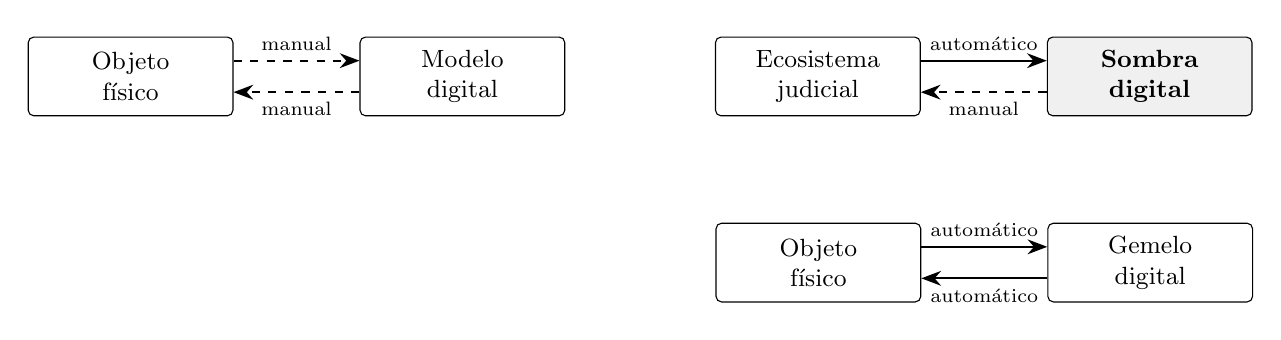
\begin{tikzpicture}[
  obj/.style={draw, rounded corners=2pt, minimum width=2.6cm, minimum height=1.0cm, align=center, font=\small},
  auto/.style={-{Stealth[length=2.5mm]}, thick},
  man/.style={-{Stealth[length=2.5mm]}, thick, dashed},
  lab/.style={font=\scriptsize, midway}]
% Digital Model
\node[obj] (p1) {Objeto\\físico};
\node[obj, right=1.6cm of p1] (v1) {Modelo\\digital};
\draw[man] ([yshift=2mm]p1.east) -- node[lab, above]{manual} ([yshift=2mm]v1.west);
\draw[man] ([yshift=-2mm]v1.west) -- node[lab, below]{manual} ([yshift=-2mm]p1.east);
% Digital Shadow
\node[obj, right=1.9cm of v1] (p2) {Ecosistema\\judicial};
\node[obj, right=1.6cm of p2, fill=gray!12] (v2) {\textbf{Sombra}\\\textbf{digital}};
\draw[auto] ([yshift=2mm]p2.east) -- node[lab, above]{automático} ([yshift=2mm]v2.west);
\draw[man] ([yshift=-2mm]v2.west) -- node[lab, below]{manual} ([yshift=-2mm]p2.east);
% Digital Twin
\node[obj, below=1.35cm of $(p2.south)!0.5!(v2.south)$, xshift=-2.1cm] (p3) {Objeto\\físico};
\node[obj, right=1.6cm of p3] (v3) {Gemelo\\digital};
\draw[auto] ([yshift=2mm]p3.east) -- node[lab, above]{automático} ([yshift=2mm]v3.west);
\draw[auto] ([yshift=-2mm]v3.west) -- node[lab, below]{automático} ([yshift=-2mm]p3.east);
\end{tikzpicture}
\caption{Clasificación de contrapartes virtuales según el flujo de información (adaptada de \cite{Kritzinger2018}). En el dominio judicial la retroalimentación automática hacia la infraestructura institucional es improcedente, por lo que la sombra digital (sombreada) es la configuración adecuada.}
\label{fig:dmdsdt}
\end{figure}

%% ============================================================
\section{Modelo Formal MALTG}
\label{sec:formal}

Esta sección formaliza el marco de evaluación. El objetivo es que la sombra digital no sea únicamente una estructura de datos, sino un artefacto \emph{medible} contra un modelo normativo de referencia.

\begin{Definition}[Ontología de referencia]
La ontología de gobernanza LegalTech es una tupla $\Omega = \langle C, P, I, \sigma \rangle$, donde $C$ es la taxonomía de clases (conceptos de TOGAF, COBIT, ITIL, NIST CSF, IA, cadena de bloques, datos abiertos, seguridad, interoperabilidad y dominio LegalTech), $P$ el conjunto de propiedades (de objeto y de anotación), $I$ el conjunto de instancias y $\sigma: C \rightarrow [0,100]$ una función de puntuación de madurez conceptual asignada por juicio experto. $\Omega$ se materializa en OWL~2 siguiendo prácticas establecidas de ingeniería ontológica \cite{Gruber1993,Uschold1996,Guarino2002}.
\end{Definition}

\begin{Definition}[Sombra digital estructural]
La sombra digital es un grafo dirigido $\Delta = G(V, E, \lambda)$ en el que $V$ es el conjunto de componentes observados del ecosistema (portales, SPA, sistemas de gestión procesal, repositorios), $E \subseteq V \times V$ el conjunto de flujos de información entre componentes y $\lambda$ una función de etiquetado que asigna a cada vértice su capa arquitectónica, su evidencia de observación y sus metadatos JSON-LD.
\end{Definition}

\begin{Definition}[Anclaje semántico]
La función de anclaje $\Gamma: V \rightarrow 2^{C}$ asocia cada componente de la sombra con los conceptos ontológicos que materializa, implementada mediante la propiedad \texttt{maltg:mapsTo} en el contexto JSON-LD. El conjunto de cobertura inducido es
\begin{equation}
R \;=\; \bigcup_{v \in V} \Gamma(v) \;\subseteq\; C .
\label{eq:coverage-set}
\end{equation}
\end{Definition}

Cada dimensión de gobernanza $d$ se especifica por un concepto raíz $r_d \in C$ y un conjunto de subconceptos $S_d = \{s_1, \dots, s_{n_d}\} \subset C$. La pregunta central de validación es: ¿en qué medida la sombra observada \emph{cubre} la dimensión $d$ prescrita por la ontología?

\begin{Definition}[Cobertura jerárquica $\Psi$]
Sean $w_r, w_s \in (0,1)$ con $w_r + w_s = 1$ los pesos del concepto raíz y de los subconceptos. La cobertura de la dimensión $d$ es
\begin{equation}
\Psi(d) \;=\; w_r \cdot \mathbb{1}\!\left[\, r_d \in R \,\right] \;+\; w_s \cdot \frac{\lvert S_d \cap R \rvert}{\lvert S_d \rvert},
\label{eq:psi}
\end{equation}
donde $\mathbb{1}[\cdot]$ es la función indicatriz. Los pesos por defecto son $(w_r, w_s) = (0{,}40,\, 0{,}60)$, calibrables mediante el proceso analítico jerárquico (AHP) \cite{Saaty1990}.
\end{Definition}

\begin{Proposition}[Propiedades de $\Psi$]
Para toda dimensión $d$: (i) $\Psi(d) \in [0,1]$; (ii) $\Psi$ es monótona no decreciente respecto a $R$, es decir, si $R \subseteq R'$ entonces $\Psi_R(d) \leq \Psi_{R'}(d)$; (iii) $\Psi(d) = 1$ si y solo si $r_d \in R$ y $S_d \subseteq R$.
\end{Proposition}

\begin{proof}
(i) es inmediata por ser combinación convexa de términos en $[0,1]$. (ii) se sigue de que tanto $\mathbb{1}[r_d \in R]$ como $\lvert S_d \cap R\rvert$ son no decrecientes bajo inclusión de conjuntos. (iii) $\Psi(d)=1$ exige que ambos sumandos alcancen su máximo, lo que ocurre exactamente cuando la raíz está cubierta y la intersección es total. \end{proof}

La puntuación ontológica de la dimensión se define como la media de madurez de sus clases puntuadas, $\mathrm{onto}(d) = \overline{\sigma}(C_d)$, y la puntuación efectiva de la sombra como su proyección por la cobertura:
\begin{equation}
\mathrm{sds}(d) \;=\; \mathrm{onto}(d) \cdot \Psi(d).
\label{eq:dtscore}
\end{equation}

\begin{Definition}[Brecha de gobernanza $\delta$]
La brecha de la dimensión $d$ es la pérdida absoluta de madurez imputable a la falta de cobertura:
\begin{equation}
\delta(d) \;=\; \mathrm{onto}(d) - \mathrm{sds}(d) \;=\; \mathrm{onto}(d)\,\bigl(1 - \Psi(d)\bigr) \;\in\; [0, \mathrm{onto}(d)].
\label{eq:delta}
\end{equation}
El ordenamiento decreciente de $\delta$ produce la agenda de remediación: la dimensión con mayor $\delta$ es el objetivo prioritario de inversión tecnológica.
\end{Definition}

La agregación global sobre el conjunto de dimensiones $D$ admite ponderación experta $\{\omega_d\}$ obtenida por consenso (p.~ej.\ Delphi/AHP \cite{Saaty1990}), con $\sum_{d \in D} \omega_d = 1$:
\begin{equation}
\mathrm{SDS}_{\mathrm{global}} = \sum_{d \in D} \omega_d \, \mathrm{sds}(d), \qquad
\mathrm{Onto}_{\mathrm{global}} = \sum_{d \in D} \omega_d \, \mathrm{onto}(d), \qquad
\Psi_{\mathrm{global}} = \frac{\mathrm{SDS}_{\mathrm{global}}}{\mathrm{Onto}_{\mathrm{global}}}.
\label{eq:global}
\end{equation}

Finalmente, el índice de madurez se interpreta mediante la función escalonada $L: [0,100] \rightarrow \{1,\dots,5\}$ de la Tabla~\ref{tab:levels}, análoga a los modelos de madurez de capacidad utilizados en gobernanza de TI \cite{DeHaes2013}. La puntuación de contenido de la ontología se apoya, para la validación por panel de expertos, en la razón de validez de contenido de Lawshe \cite{Lawshe1975}, $\mathrm{CVR} = (n_e - N/2)/(N/2)$, donde $n_e$ es el número de expertos que califican un concepto como esencial y $N$ el total del panel.

\begin{table}[H]
\caption{Escala de niveles de madurez LegalTech empleada por la función $L$.}
\label{tab:levels}
\begin{tabularx}{\textwidth}{clcX}
\toprule
\textbf{Nivel} & \textbf{Denominación} & \textbf{Rango} & \textbf{Caracterización}\\
\midrule
1 & Inicial & 0--20 & Procesos manuales o ad hoc, sin estructura digital.\\
2 & En transición & 21--40 & Islas digitales, datos en silos, sin interoperabilidad.\\
3 & Definido & 41--60 & Procesos definidos y portales modernos emergentes; brechas de ejecución.\\
4 & Gestionado & 61--80 & Servicios medidos, API e integración semántica parcial.\\
5 & Optimizado & 81--100 & Ecosistema interoperable, datos enlazados y mejora continua.\\
\bottomrule
\end{tabularx}
\end{table}

\textbf{Complejidad.} El cómputo de $R$ requiere $O(|V| \cdot k)$ operaciones, con $k$ el número medio de referencias semánticas por componente, y la evaluación de las ecuaciones \eqref{eq:psi}--\eqref{eq:global} es $O\!\left(\sum_{d} |S_d|\right)$; la validación completa es lineal en el tamaño de la sombra y de la ontología, lo que habilita su ejecución en cada ciclo de ingesta sin penalización perceptible.

%% ============================================================
\section{Arquitectura MALTG-SDS y Módulo GET-SDS}
\label{sec:arch}

\subsection{Vista General}
La arquitectura (Figura~\ref{fig:arch}) se organiza en cuatro capas desacopladas y desplegadas como contenedores Docker: (i) \textbf{capa de adquisición}, que ejecuta el protocolo de observación web; (ii) \textbf{capa semántica}, que mantiene la ontología $\Omega$ en OWL~2 y produce la sombra $\Delta$ en JSON-LD; (iii) \textbf{capa de validación}, que computa $\Psi$, $\delta$ y el índice de madurez; y (iv) \textbf{capa de presentación}, que expone la sombra mediante una API REST (FastAPI) y una interfaz de exploración con un grafo tridimensional interactivo (Three.js) en el que los nodos ontológicos se representan como estrellas y las capas arquitectónicas como constelaciones; el resultado del escaneo enciende o atenúa cada estrella según exista evidencia observada, proporcionando una metáfora visual inmediata del estado de cobertura.

\begin{figure}[H]
\centering
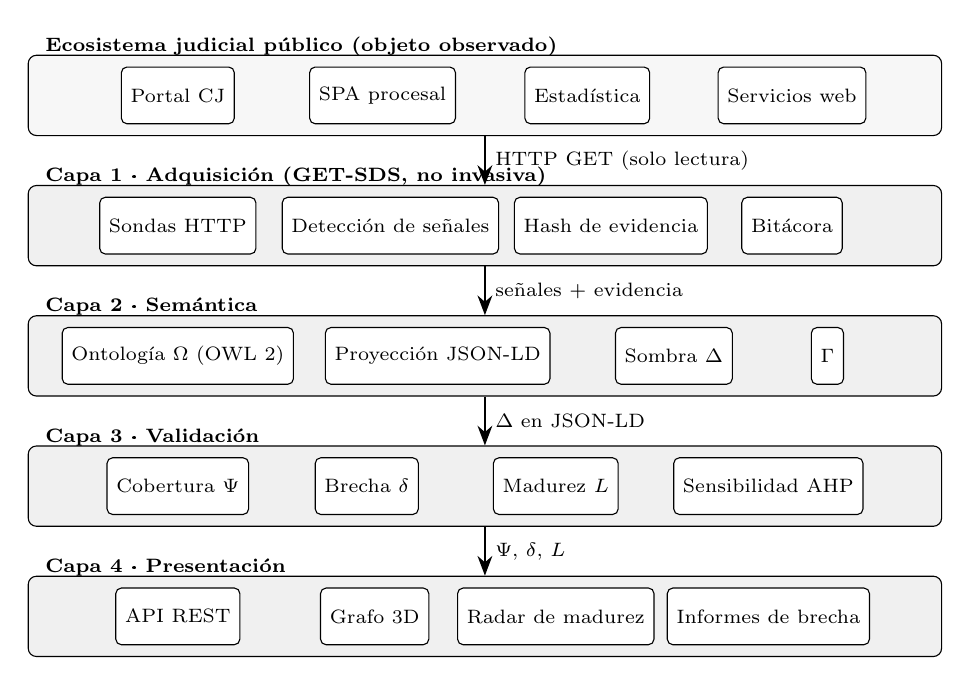
\begin{tikzpicture}[
  capa/.style={draw, rounded corners=3pt, minimum width=11.6cm, minimum height=1.02cm, align=center, font=\small},
  comp/.style={draw, rounded corners=2pt, minimum height=0.72cm, align=center, font=\scriptsize, fill=white},
  flow/.style={-{Stealth[length=2.5mm]}, thick},
  node distance=0.42cm]
\node[capa, fill=gray!6]  (l1) {};
\node[comp] at ($(l1.center)+(-3.9,0)$) {Portal CJ};
\node[comp] at ($(l1.center)+(-1.3,0)$) {SPA procesal};
\node[comp] at ($(l1.center)+(1.3,0)$)  {Estadística};
\node[comp] at ($(l1.center)+(3.9,0)$)  {Servicios web};
\node[font=\scriptsize\bfseries, anchor=west] at ($(l1.west)+(0.1,0.62)$) {Ecosistema judicial público (objeto observado)};

\node[capa, below=0.62cm of l1, fill=gray!12] (l2) {};
\node[comp] at ($(l2.center)+(-3.9,0)$) {Sondas HTTP};
\node[comp] at ($(l2.center)+(-1.2,0)$) {Detección de señales};
\node[comp] at ($(l2.center)+(1.6,0)$)  {Hash de evidencia};
\node[comp] at ($(l2.center)+(3.9,0)$)  {Bitácora};
\node[font=\scriptsize\bfseries, anchor=west] at ($(l2.west)+(0.1,0.62)$) {Capa 1 · Adquisición (GET-SDS, no invasiva)};

\node[capa, below=0.62cm of l2, fill=gray!12] (l3) {};
\node[comp] at ($(l3.center)+(-3.9,0)$) {Ontología $\Omega$ (OWL 2)};
\node[comp] at ($(l3.center)+(-0.6,0)$)  {Proyección JSON-LD};
\node[comp] at ($(l3.center)+(2.4,0)$)  {Sombra $\Delta$};
\node[comp] at ($(l3.center)+(4.35,0)$)  {$\Gamma$};
\node[font=\scriptsize\bfseries, anchor=west] at ($(l3.west)+(0.1,0.62)$) {Capa 2 · Semántica};

\node[capa, below=0.62cm of l3, fill=gray!12] (l4) {};
\node[comp] at ($(l4.center)+(-3.9,0)$) {Cobertura $\Psi$};
\node[comp] at ($(l4.center)+(-1.5,0)$) {Brecha $\delta$};
\node[comp] at ($(l4.center)+(0.9,0)$)  {Madurez $L$};
\node[comp] at ($(l4.center)+(3.6,0)$)  {Sensibilidad AHP};
\node[font=\scriptsize\bfseries, anchor=west] at ($(l4.west)+(0.1,0.62)$) {Capa 3 · Validación};

\node[capa, below=0.62cm of l4, fill=gray!12] (l5) {};
\node[comp] at ($(l5.center)+(-3.9,0)$) {API REST};
\node[comp] at ($(l5.center)+(-1.4,0)$) {Grafo 3D};
\node[comp] at ($(l5.center)+(0.9,0)$)  {Radar de madurez};
\node[comp] at ($(l5.center)+(3.6,0)$)  {Informes de brecha};
\node[font=\scriptsize\bfseries, anchor=west] at ($(l5.west)+(0.1,0.62)$) {Capa 4 · Presentación};

\draw[flow] (l1) -- node[right, font=\scriptsize]{HTTP GET (solo lectura)} (l2);
\draw[flow] (l2) -- node[right, font=\scriptsize]{señales + evidencia} (l3);
\draw[flow] (l3) -- node[right, font=\scriptsize]{$\Delta$ en JSON-LD} (l4);
\draw[flow] (l4) -- node[right, font=\scriptsize]{$\Psi$, $\delta$, $L$} (l5);
\end{tikzpicture}
\caption{Arquitectura de referencia MALTG-SDS. El flujo es unidireccional desde el ecosistema observado hacia la presentación, en coherencia con la definición de sombra digital: no existe actuación automática sobre la infraestructura institucional.}
\label{fig:arch}
\end{figure}

\subsection{Protocolo de Adquisición No Invasivo}
El módulo GET-SDS ejecuta sondas HTTP de solo lectura contra un conjunto configurable de objetivos públicos (portal principal, sistema de consulta procesal, subportal estadístico). Siguiendo las recomendaciones ético-legales de la literatura \cite{Krotov2020}, el agente (i) se identifica con un \emph{User-Agent} explícito con propósito declarado, (ii) accede únicamente a recursos públicos sin autenticación, (iii) no envía formularios ni ejecuta acciones de escritura, y (iv) registra cada captura con marca temporal y suma de verificación criptográfica para garantizar trazabilidad probatoria. Sobre las respuestas se computan \emph{señales} deterministas mediante análisis del marcado: tecnología generadora (p.~ej.\ gestor de contenido), presencia de enlaces heredados (extensiones JSF/PHP), confirmación de SPA, referencias a políticas de datos abiertos y de integridad, y —crucialmente— presencia o ausencia de datos estructurados incrustados (JSON-LD/\texttt{schema.org} \cite{Guha2016}) y de API pública documentada.

\subsection{Proyección Semántica a JSON-LD}
Las señales se proyectan a una instancia JSON-LD cuya cabecera \texttt{@context} (Tabla~\ref{tab:context}) reutiliza vocabularios estándar (Dublin Core, SKOS, Schema.org) y define el espacio de nombres propio \texttt{maltg:} para los términos de gobernanza. La elección de JSON-LD obedece a tres criterios derivados de la literatura: compatibilidad nativa con el ecosistema de desarrollo web \cite{Guha2016}, condición de puerta de entrada al modelo de datos enlazados \cite{Bizer2009,Hitzler2021} y alineación con los principios FAIR de interoperabilidad y reutilización \cite{Wilkinson2016}. Cada componente detectado se serializa con su capa, su evidencia (URL, estado HTTP, tamaño, latencia), sus hallazgos y brechas, y su anclaje $\Gamma$ mediante \texttt{maltg:mapsTo}, lo que convierte la sombra en un subgrafo de conocimiento consultable \cite{Hogan2021}.

\begin{table}[H]
\caption{Contexto JSON-LD de la sombra digital (extracto). Los términos del artefacto se resuelven a IRI de vocabularios estándar o del espacio de nombres propio.}
\label{tab:context}
\begin{tabularx}{\textwidth}{llX}
\toprule
\textbf{Término} & \textbf{IRI / Prefijo} & \textbf{Función semántica}\\
\midrule
\texttt{maltg:} & \texttt{http://maltg.arch/onto\#} & Ontología de gobernanza LegalTech (clases y propiedades).\\
\texttt{sdt:} & \texttt{http://maltg.arch/sdt\#} & Vocabulario estructural de la sombra (componentes, flujos).\\
\texttt{schema:} & \texttt{http://schema.org/} & Interoperabilidad con datos estructurados web \cite{Guha2016}.\\
\texttt{dcterms:} & \texttt{http://purl.org/dc/terms/} & Metadatos de título y descripción.\\
\texttt{skos:} & \texttt{http://www.w3.org/2004/02/skos/core\#} & Etiquetado preferente de conceptos.\\
\texttt{score} & \texttt{maltg:maturityScore} & Puntuación de madurez $\sigma$ del componente o dimensión.\\
\texttt{evidence} & \texttt{sdt:evidence} & Evidencia de observación (URL, estado, latencia, hash).\\
\texttt{maltg\_ref} & \texttt{maltg:mapsTo} (\texttt{@type=@id}) & Anclaje semántico $\Gamma$ hacia conceptos de $\Omega$.\\
\texttt{services} & \texttt{sdt:hasComponent} & Vértices $V$ del grafo $\Delta$.\\
\texttt{connections} & \texttt{sdt:hasFlow} & Aristas $E$ del grafo $\Delta$.\\
\bottomrule
\end{tabularx}
\end{table}

\subsection{Ciclo de Evaluación y Visualización}
Tras cada ingesta, la capa de validación computa las ecuaciones \eqref{eq:coverage-set}--\eqref{eq:global} y persiste la sombra fechada, lo que produce una serie temporal de artefactos comparables entre instituciones y entre fechas. El diseño del ciclo se inspira en el bucle MAPE-K de la computación autonómica \cite{Kephart2003} —monitorizar, analizar, planificar y ejecutar sobre una base de conocimiento compartida— con la salvedad deliberada de que la fase de ejecución se restringe a recomendaciones: el cierre del lazo sobre el sistema observado corresponde a la institución. Esta restricción es la traducción arquitectónica del carácter de \emph{sombra} (y no gemelo) del artefacto \cite{Kritzinger2018,Sepasgozar2021}.

%% ============================================================
\section{Caso de Estudio y Resultados}
\label{sec:results}

\subsection{Diseño Experimental}
La validación empírica comprende dos escenarios complementarios. El \textbf{Escenario A} aplica el módulo GET-SDS al ecosistema digital público del Consejo de la Judicatura del Ecuador (\texttt{funcionjudicial.gob.ec}), generando la sombra \texttt{LegalTech\_funcionjudicial} con cuatro dimensiones de madurez orientadas a diagnóstico institucional. El \textbf{Escenario B} valida el motor $\Psi$/$\delta$ sobre una sombra sintética de 39 componentes anclada a la ontología completa (131 nodos, 144 relaciones, de las cuales 14 son transversales), evaluando las diez dimensiones de gobernanza del marco MALTG.

\subsection{Escenario A: Sombra Digital del Consejo de la Judicatura}
La Tabla~\ref{tab:signals} resume las señales de observación obtenidas en la ingesta del 8 de julio de 2026. La sombra resultante contiene 34 componentes, 32 flujos y 7 capas arquitectónicas. Tres hallazgos estructurales destacan: la coexistencia de un portal moderno sobre gestor de contenido genérico con 19 enlaces a aplicaciones heredadas (6 JSF y 13 PHP); la confirmación de una SPA de consulta procesal sin API pública documentada; y la ausencia total de datos estructurados JSON-LD en el marcado, pese a la existencia de referencias declarativas a políticas de datos abiertos —el patrón exacto de brecha entre publicación nominal y reutilización efectiva descrito por la literatura de gobierno abierto \cite{Janssen2012,Attard2015}.

\begin{table}[H]
\caption{Señales de observación del ecosistema del Consejo de la Judicatura (ingesta del 8 de julio de 2026; agente identificado, solo lectura).}
\label{tab:signals}
\begin{tabularx}{\textwidth}{Xcc}
\toprule
\textbf{Señal} & \textbf{Valor} & \textbf{Implicación de gobernanza}\\
\midrule
Portal en línea (HTTP 200) & Sí & Disponibilidad del canal ciudadano.\\
Gestor de contenido genérico confirmado & Sí & Dependencia de plataforma no especializada.\\
Enlaces heredados JSF & 6 & Deuda técnica visible en superficie pública.\\
Enlaces heredados PHP & 13 & Fragmentación tecnológica.\\
SPA de consulta procesal confirmada & Sí & Modernización parcial del front-end.\\
Referencia a datos abiertos & Sí & Compromiso declarativo presente.\\
Referencia a norma antisoborno (ISO 37001) & Sí & Señal de cumplimiento declarativo.\\
JSON-LD / \texttt{schema.org} detectado & \textbf{No} & Ausencia de web semántica.\\
API pública documentada & \textbf{No} & Bloqueo de reutilización programática.\\
\bottomrule
\end{tabularx}
\end{table}

La evaluación multidimensional (Tabla~\ref{tab:cjdims}, Figura~\ref{fig:radar}) arroja un índice global de madurez de \textbf{46/100}, que la función $L$ sitúa en el nivel 3 («Definido») de la Tabla~\ref{tab:levels}. La dimensión más débil es la capa de datos e interoperabilidad semántica (28/100), consistente con las señales negativas de JSON-LD y API; la más fuerte es el cumplimiento regulatorio declarativo (58/100), impulsada por las referencias normativas detectadas.

\begin{table}[H]
\caption{Dimensiones de madurez de la sombra digital del Consejo de la Judicatura.}
\label{tab:cjdims}
\begin{tabularx}{\textwidth}{Xccc}
\toprule
\textbf{Dimensión} & \textbf{Puntuación} & \textbf{Hallazgos} & \textbf{Brechas}\\
\midrule
Capa de datos e interoperabilidad semántica & 28 & 2 & 3\\
Arquitectura de integración (API y front-end) & 42 & 2 & 3\\
Transformación e innovación declarada & 55 & 2 & 2\\
Cumplimiento regulatorio y automatización & 58 & 3 & 2\\
\midrule
\textbf{Índice global (media)} & \textbf{46} & \multicolumn{2}{c}{Nivel 3 · Definido}\\
\bottomrule
\end{tabularx}
\end{table}

\begin{figure}[H]
\centering
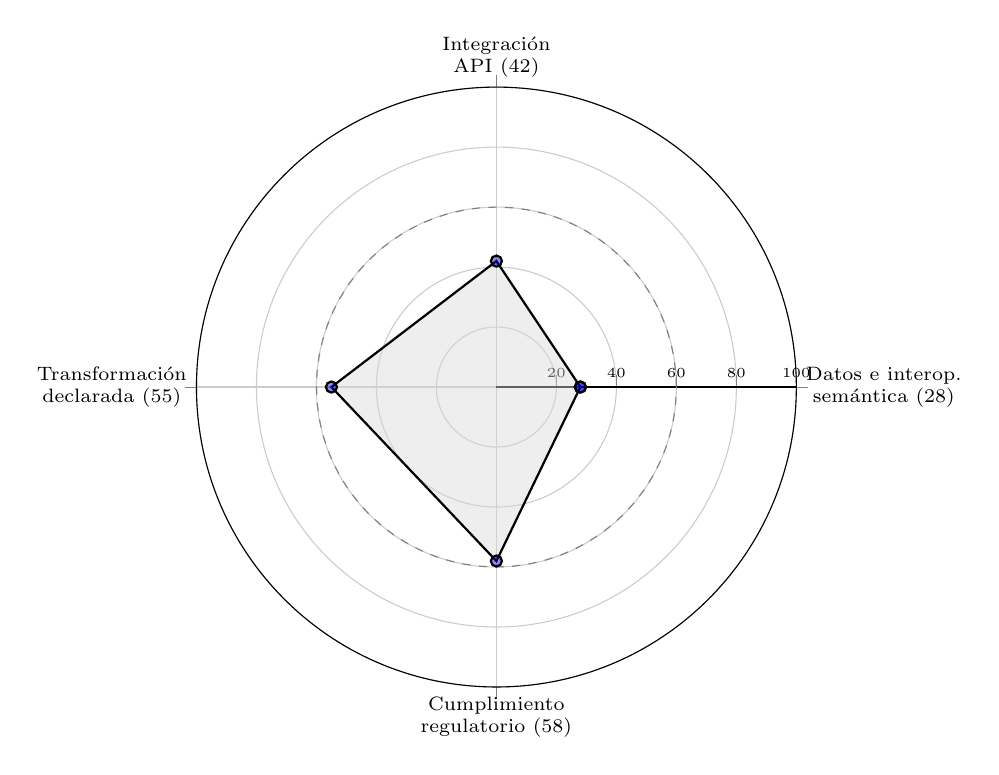
\begin{tikzpicture}
\begin{polaraxis}[
  width=9.2cm,
  xtick={0,90,180,270},
  xticklabels={
    {Datos e interop.\\semántica (28)},
    {Integración\\API (42)},
    {Transformación\\declarada (55)},
    {Cumplimiento\\regulatorio (58)}},
  xticklabel style={font=\scriptsize, align=center},
  ytick={20,40,60,80,100},
  yticklabel style={font=\tiny},
  ymin=0, ymax=100,
  grid=both,
  major grid style={gray!40},
]
\addplot+[thick, mark=*, fill=gray!30, fill opacity=0.45, draw=black]
  coordinates {(0,28) (90,42) (180,55) (270,58) (360,28)};
\addplot+[dashed, no marks, domain=0:360, samples=73, draw=gray]{60};
\end{polaraxis}
\end{tikzpicture}
\caption{Radar de madurez de las cuatro dimensiones del Consejo de la Judicatura. La línea discontinua marca el umbral del nivel 4 («Gestionado», 61+). El polígono observado (46/100 en promedio) evidencia el rezago de la interoperabilidad semántica.}
\label{fig:radar}
\end{figure}

\subsection{Escenario B: Validación de Cobertura de Diez Dimensiones}
La Tabla~\ref{tab:validation} y la Figura~\ref{fig:gaps} presentan la validación del motor formal sobre la sombra sintética. La cobertura global asciende a $\Psi_{\mathrm{global}} = 66{,}9/73{,}9 = 0{,}905$: la sombra materializa el 90{,}5\% de la madurez prescrita por la ontología. Seis dimensiones alcanzan cobertura total ($\Psi = 1$), mientras que la brecha máxima corresponde al dominio LegalTech ($\delta = 30{,}2$; $\Psi = 0{,}60$), cuya raíz ontológica no está cubierta por ningún componente ($\mathbb{1}[r_d \in R] = 0$), seguida de la gobernanza TOGAF ($\delta = 18{,}1$), donde faltan los subconceptos del ciclo ADM, y de la integración de IA ($\delta = 14{,}5$). El ordenamiento por $\delta$ produce directamente la agenda de remediación prevista por la ecuación \eqref{eq:delta}.

\begin{table}[H]
\caption{Validación de cobertura jerárquica por dimensión (Escenario B). $\mathrm{onto}(d)$: madurez ontológica; $\Psi(d)$: cobertura; $\mathrm{sds}(d)$: madurez efectiva de la sombra; $\delta(d)$: brecha; $(w_r,w_s)=(0{,}40,\,0{,}60)$.}
\label{tab:validation}
\begin{tabularx}{\textwidth}{Xccccc}
\toprule
\textbf{Dimensión} & $\mathbf{onto(d)}$ & $\mathbf{\Psi(d)}$ & $\mathbf{sds(d)}$ & $\boldsymbol{\delta}\mathbf{(d)}$ & \textbf{Subconceptos faltantes}\\
\midrule
Gobernanza TOGAF & 60{,}3 & 0{,}70 & 42{,}2 & 18{,}1 & 3 de 6\\
Control COBIT & 62{,}7 & 1{,}00 & 62{,}7 & 0{,}0 & 0 de 5\\
Gestión de servicios ITIL & 79{,}5 & 1{,}00 & 79{,}5 & 0{,}0 & 0 de 5\\
Resiliencia NIST CSF & 72{,}0 & 1{,}00 & 72{,}0 & 0{,}0 & 0 de 5\\
Integración de IA & 96{,}9 & 0{,}85 & 82{,}4 & 14{,}5 & 1 de 4\\
Cadena de bloques & 52{,}4 & 0{,}85 & 44{,}5 & 7{,}9 & 1 de 4\\
Datos abiertos & 78{,}5 & 1{,}00 & 78{,}5 & 0{,}0 & 0 de 4\\
Postura de seguridad & 80{,}4 & 1{,}00 & 80{,}4 & 0{,}0 & 0 de 4\\
Interoperabilidad & 81{,}2 & 1{,}00 & 81{,}2 & 0{,}0 & 0 de 8\\
Dominio LegalTech & 75{,}5 & 0{,}60 & 45{,}3 & 30{,}2 & raíz no cubierta\\
\midrule
\textbf{Global (media simple)} & \textbf{73{,}9} & \textbf{0{,}905} & \textbf{66{,}9} & \textbf{7{,}0} & ---\\
\bottomrule
\end{tabularx}
\end{table}

\begin{figure}[H]
\centering
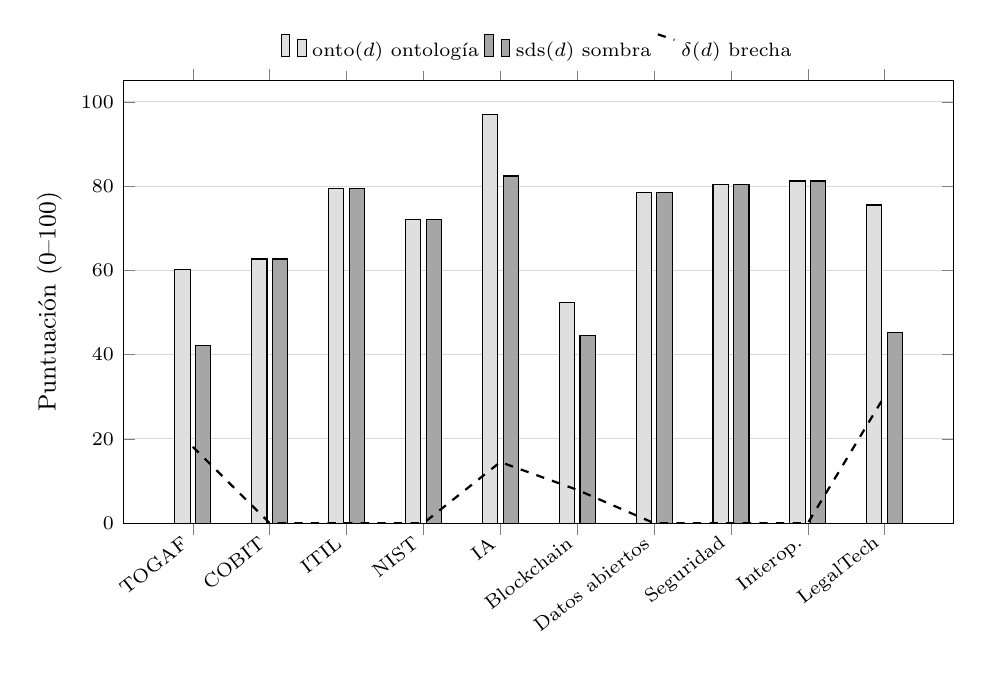
\begin{tikzpicture}
\begin{axis}[
  ybar,
  width=\textwidth, height=7.2cm,
  bar width=5.5pt,
  ymin=0, ymax=105,
  ylabel={Puntuación (0--100)},
  ylabel style={font=\small},
  symbolic x coords={TOGAF,COBIT,ITIL,NIST,IA,Blockchain,Datos abiertos,Seguridad,Interop.,LegalTech},
  xtick=data,
  x tick label style={rotate=38, anchor=east, font=\scriptsize},
  ytick={0,20,40,60,80,100},
  yticklabel style={font=\scriptsize},
  legend style={font=\scriptsize, at={(0.5,1.02)}, anchor=south, legend columns=3, draw=none},
  ymajorgrids, major grid style={gray!30},
]
\addplot+[draw=black, fill=gray!25] coordinates
  {(TOGAF,60.3) (COBIT,62.7) (ITIL,79.5) (NIST,72.0) (IA,96.9) (Blockchain,52.4) (Datos abiertos,78.5) (Seguridad,80.4) (Interop.,81.2) (LegalTech,75.5)};
\addplot+[draw=black, fill=gray!70] coordinates
  {(TOGAF,42.2) (COBIT,62.7) (ITIL,79.5) (NIST,72.0) (IA,82.4) (Blockchain,44.5) (Datos abiertos,78.5) (Seguridad,80.4) (Interop.,81.2) (LegalTech,45.3)};
\addplot[sharp plot, thick, dashed, black] coordinates
  {(TOGAF,18.1) (COBIT,0) (ITIL,0) (NIST,0) (IA,14.5) (Blockchain,7.9) (Datos abiertos,0) (Seguridad,0) (Interop.,0) (LegalTech,30.2)};
\legend{$\mathrm{onto}(d)$ ontología, $\mathrm{sds}(d)$ sombra, $\delta(d)$ brecha}
\end{axis}
\end{tikzpicture}
\caption{Madurez ontológica frente a madurez efectiva de la sombra por dimensión (Escenario B). La línea discontinua traza la brecha $\delta(d)$; el dominio LegalTech y la gobernanza TOGAF concentran la agenda de remediación.}
\label{fig:gaps}
\end{figure}

\subsection{Análisis de Sensibilidad}
Dado que $\Psi$ depende de los pesos $(w_r, w_s)$, se evaluó la robustez del ordenamiento de brechas perturbando $w_r \in [0{,}10,\, 0{,}90]$. Por la ecuación \eqref{eq:psi}, $\Psi(d)$ es lineal en $w_r$ para cada dimensión, de modo que el orden relativo de $\delta$ solo puede alterarse en los cruces de rectas. En el Escenario B, el dominio LegalTech permanece como brecha máxima en todo el intervalo —su déficit proviene de la raíz no cubierta, que pondera exactamente $w_r$— y TOGAF conserva el segundo lugar para $w_r \leq 0{,}62$. La agenda de remediación resulta, por tanto, estable frente a variaciones razonables del juicio experto, lo que refuerza la utilidad práctica de la calibración AHP \cite{Saaty1990}.

%% ============================================================
\section{Discusión}
\label{sec:discussion}

\textbf{Implicaciones para la gobernanza judicial.} Los resultados del Escenario A convierten una intuición cualitativa —«el portal es moderno pero el ecosistema está fragmentado»— en un diagnóstico cuantitativo, fechado y reproducible: madurez 46/100 con déficit crítico de interoperabilidad semántica (28/100). Que la señal más deficitaria sea precisamente la ausencia de JSON-LD y de API pública tiene una lectura reflexiva: la institución observada carece del mismo instrumento (datos estructurados) que la sombra digital utiliza para representarla. La adopción institucional de marcado semántico, además de mejorar la encontrabilidad \cite{Guha2016}, elevaría de forma directa la dimensión más débil del radar y habilitaría a terceros —academia, sociedad civil— para construir servicios de valor sobre los datos judiciales \cite{Attard2015}, en línea con los principios FAIR \cite{Wilkinson2016}.

\textbf{Contribución al problema abierto de validación semántica.} La revisión de Karabulut et al.\ identifica la ausencia de métodos para verificar que un gemelo digital efectivamente materializa su modelo semántico \cite{Karabulut2024}. La función $\Psi$ ofrece una respuesta operativa: al ser computable en tiempo lineal, acotada, monótona e interpretable dimensión a dimensión, permite auditorías continuas del alineamiento ontología--artefacto, y su descomposición raíz/subconceptos localiza el origen del déficit (concepto ausente frente a cobertura parcial), como ilustra el contraste entre LegalTech ($\mathbb{1}[r_d \in R]=0$) y TOGAF (raíz cubierta, ciclo ADM ausente) en la Tabla~\ref{tab:validation}.

\textbf{Generalización.} Aunque el caso de estudio es ecuatoriano, ningún elemento de la arquitectura es específico del país: la ontología codifica marcos internacionales (TOGAF, COBIT, ITIL, NIST CSF), el protocolo de adquisición opera sobre HTTP estándar y el contexto JSON-LD reutiliza vocabularios globales. La generación de sombras fechadas por institución habilita, como línea natural, la comparación longitudinal (evolución de una judicatura) y transversal (ranking regional de madurez LegalTech), extendiendo al sector justicia la lógica de los gemelos urbanos comparables \cite{Shahat2021}.

\textbf{Limitaciones y amenazas a la validez.} Primero, la sombra observa únicamente la superficie pública del ecosistema; sistemas internos no expuestos quedan fuera del alcance, por lo que las puntuaciones deben interpretarse como madurez \emph{observable}, cota inferior de la madurez real. Segundo, las puntuaciones ontológicas $\sigma$ y los pesos $(w_r, w_s, \omega_d)$ incorporan juicio experto; se mitigan con CVR de Lawshe \cite{Lawshe1975}, calibración AHP \cite{Saaty1990} y el análisis de sensibilidad presentado, pero no se eliminan. Tercero, el Escenario B emplea una sombra sintética para ejercitar las diez dimensiones del motor formal; la validación con múltiples instituciones reales es trabajo en curso. Cuarto, la detección de señales depende de la estabilidad del marcado de los portales; el registro criptográfico de evidencia atenúa, aunque no anula, el riesgo de deriva del observador.

%% ============================================================
\section{Conclusiones y Trabajo Futuro}
\label{sec:conclusions}

Este artículo presentó MALTG-SDS, la primera arquitectura —hasta donde conocemos— que instancia el paradigma de sombra digital sobre el ecosistema tecnológico de una institución judicial, con tres propiedades distintivas: generación automática desde evidencia web pública, fundamentación semántica en una ontología de gobernanza multiestándar serializada en JSON-LD, y validación cuantitativa mediante las funciones de cobertura jerárquica $\Psi$ y brecha $\delta$, cuyas propiedades formales se demostraron. El caso de estudio del Consejo de la Judicatura del Ecuador produjo un diagnóstico accionable (madurez 46/100, nivel 3, con la interoperabilidad semántica como prioridad de remediación), y la validación sintética de diez dimensiones exhibió una cobertura global del 90{,}5\% con una agenda de brechas estable ante perturbaciones de los pesos.

El trabajo futuro se orienta en cuatro direcciones: (i) estudios multi-institucionales y longitudinales que exploten la comparabilidad de las sombras fechadas; (ii) cierre asistido del lazo mediante recomendaciones generadas sobre la base de conocimiento, preservando la decisión humana conforme al esquema MAPE-K \cite{Kephart2003}; (iii) enriquecimiento del anclaje $\Gamma$ con técnicas de alineamiento ontológico automático sobre grafos de conocimiento \cite{Hogan2021}; y (iv) integración de indicadores empíricos de desempeño procesal —tiempos, congestión, cumplimiento de plazos— como dimensión adicional del radar, conectando la sombra estructural con el comportamiento observable del sistema de justicia \cite{Medvedeva2020}.

\vspace{6pt}

\authorcontributions{Conceptualización, metodología, software, validación, redacción: P.M.A. El autor ha leído y aceptado la versión publicada del manuscrito.}

\funding{Esta investigación no recibió financiación externa.}

\institutionalreview{No aplicable.}

\informedconsent{No aplicable.}

\dataavailability{El código fuente de la plataforma MALTG, la ontología OWL y las sombras digitales JSON-LD generadas están disponibles a solicitud al autor de correspondencia. Los datos observados proceden de recursos públicos del Consejo de la Judicatura del Ecuador.}

\conflictsofinterest{El autor declara no tener conflictos de interés.}

%% ============================================================
\begin{adjustwidth}{-\extralength}{0cm}
\reftitle{Referencias}
\bibliography{references}
\end{adjustwidth}

\end{document}
